\vspace{-0.8em}
\section{Introduction}
\label{sec:intro}

\subsection{Real-time Monocular Dense SLAM}
Simultaneous Localization and Mapping (SLAM) jointly estimates an agent's pose and the surrounding 3D scene from sensor observations. In the monocular dense setting, a single RGB camera is used to reconstruct a continuous 3D map, enabling both geometric accuracy and visual realism. The camera poses and dense reconstruction outputs underpin downstream tasks~\cite{sengupta2013urban,armeni2019scenegraph,miao2024scenegraphloc,miao2024volumetric,halacheva2024holistic} such as semantic perception, object interaction, and scene editing, and are crucial for applications in VR/AR, robotics, and autonomous driving, where accurate, low-latency 3D perception is essential.



\subsection{Related Work}
\label{sec:related_work}
\boldparagraph{Classical Visual SLAM}
Classical visual SLAM methods can be broadly categorized into two types. The first, similar to incremental SfM~\cite{agarwal2011building,schonberger2016structure,liu2024robust}, is feature-based SLAM~\cite{davison2007monoslam,mur2015orb,mur2017orb,campos2021orb}, relying on keypoint extraction and descriptor matching to provide constraints for triangulation and PnP~\cite{lepetit2009ep,kneip2011novel} pose estimation. The second, known as direct methods, such as LSD-SLAM~\cite{engel2014lsd} and DSO~\cite{engel2017direct}, optimizes camera poses by minimizing photometric error from pixel intensities while estimating a per-frame depth map. Both categories typically adopt a frontend (feature-based or direct) and a backend for optimization, most often bundle adjustment~\cite{triggs1999bundle} to jointly refine poses and structure. However, they rely heavily on accurate camera calibration and are generally limited to sparse 3D reconstructions.

\boldparagraph{Dense Visual SLAM}
% To enable denser reconstructions, deep learning techniques have been incorporated into either the frontend or the scene representation.
% DROID-SLAM~\cite{teed2021droid} employs RAFT~\cite{teed2020raft} to obtain dense optical flow for dense correspondences in the frontend, and performs dense bundle adjustment on the GPU using CUDA in the backend.
% SuperPrimitive~\cite{mazur2024superprimitive} and COMO~\cite{dexheimer2024compact} leverage monocular priors, such as surface normals and depth distribution, from off-the-shelf pretrained models, and adopt a direct photometric loss for optimization.
% Back-on-Track~\cite{chen2025back} uses a point tracker for correspondences, and in the backend, optimizes a scale grid to deform the mono depth prior.
% NICER-SLAM~\cite{zhu2024nicer} and MonoGS~\cite{matsuki2024gaussian} use NeRF~\cite{mildenhall2021nerf} and 3DGS~\cite{kerbl20233dgs}, respectively, as scene representations. They optimize both camera poses and the 3D scene using a rendering loss.
% To further enhance tracking robustness and geometric accuracy, methods such as GlORIE-SLAM~\cite{zhang2024glorie} and Splat-SLAM~\cite{sandstrom2025splat}, among others~\cite{zhang2023go,zhang2023hi,zhang2024hi}, incorporate additional tracking modules and monocular depth priors into the neural SLAM pipeline.
To enable denser reconstructions, recent works have incorporated deep learning into either the frontend or the scene representation. For example, DROID-SLAM~\cite{teed2021droid} uses RAFT~\cite{teed2020raft} for dense optical flow in the frontend and performs dense bundle adjustment on the GPU, while methods such as SuperPrimitive~\cite{mazur2024superprimitive} and COMO~\cite{dexheimer2024compact} leverage monocular priors (e.g., surface normals, depth distributions) from pretrained models with direct photometric optimization. BA-Track~\cite{chen2025back} augments point-based tracking with a scale-grid deformation of monocular depth priors. Neural scene representations have also been adopted, with NICER-SLAM~\cite{zhu2024nicer} and MonoGS~\cite{matsuki2024gaussian} optimizing camera poses and 3D structure using NeRF~\cite{mildenhall2021nerf} and 3D Gaussian Splatting~\cite{kerbl20233dgs}, respectively. Tracking robustness and geometric accuracy have been further improved by integrating depth priors and auxiliary trackers~\cite{zhang2024glorie,sandstrom2025splat,zhang2023go,zhang2023hi,zhang2024hi}. However, most approaches still require accurate camera intrinsics and many struggle to achieve true real-time performance due to the computational demands of dense optimization and neural rendering.



\boldparagraph{SLAM with 3D Foundation Models}
All aforementioned methods require known and accurate camera intrinsics. With the advent of 3D foundation models~\cite{dust3r,mast3r,wang2025vggt}, several intrinsic-free SLAM frameworks have emerged, aiming to produce dense outputs without calibration. Methods such as Spann3R~\cite{wang2025spann3r} and others~\cite{liu2025slam3r,wang2025cut3r,cabon2025must3r} extend the two-view DUSt3R~\cite{dust3r} model to sequential inputs, directly regressing point clouds in a unified global coordinate system. Reloc3r~\cite{dong2025reloc3r} instead regresses only relative poses and performs offline global optimization using SfM techniques~\cite{pan2024glomap,sweeney2015theia,zhang2023revisiting}. MASt3R-SLAM~\cite{murai2025mast3rslam} extracts dense correspondences from MASt3R~\cite{mast3r} and feeds them into a classical optimization pipeline, while submap-based methods~\cite{maggio2025vggtslam,deng2025vggtlong} employs the multiview model VGGT~\cite{wang2025vggt} to regress local submaps before stitching them via pose graph optimization.
While these approaches address some classical limitations, they still face notable drawbacks:
\begin{enumerate}[label=\arabic*., leftmargin=*, itemsep=0em, parsep=0pt, topsep=0pt]
    \item Current two-view models~\cite{dust3r,mast3r} use asymmetric architectures that regress pointmaps of both views to the first view's coordinates, making it difficult to decouple views for backend optimization (\eg loop closure).
    \item Pure regression methods~\cite{wang2025spann3r,wang2025cut3r,liu2025slam3r} predict incoming frames with previous memory, but suffer from drift and start forgetting once the trajectory gets longer.
    \item Methods~\cite{wang2025spann3r,wang2025cut3r,liu2025slam3r,murai2025mast3rslam} built on current two-view models inherit the asymmetric architecture with two separate decoders, resulting in large model size. Submap-based methods~\cite{maggio2025vggtslam,deng2025vggtlong} employ an even larger multiview model~\cite{wang2025vggt} to build submaps, which further increases the size of the frontend model.
\end{enumerate}




\begin{figure*}[!t]
\centering
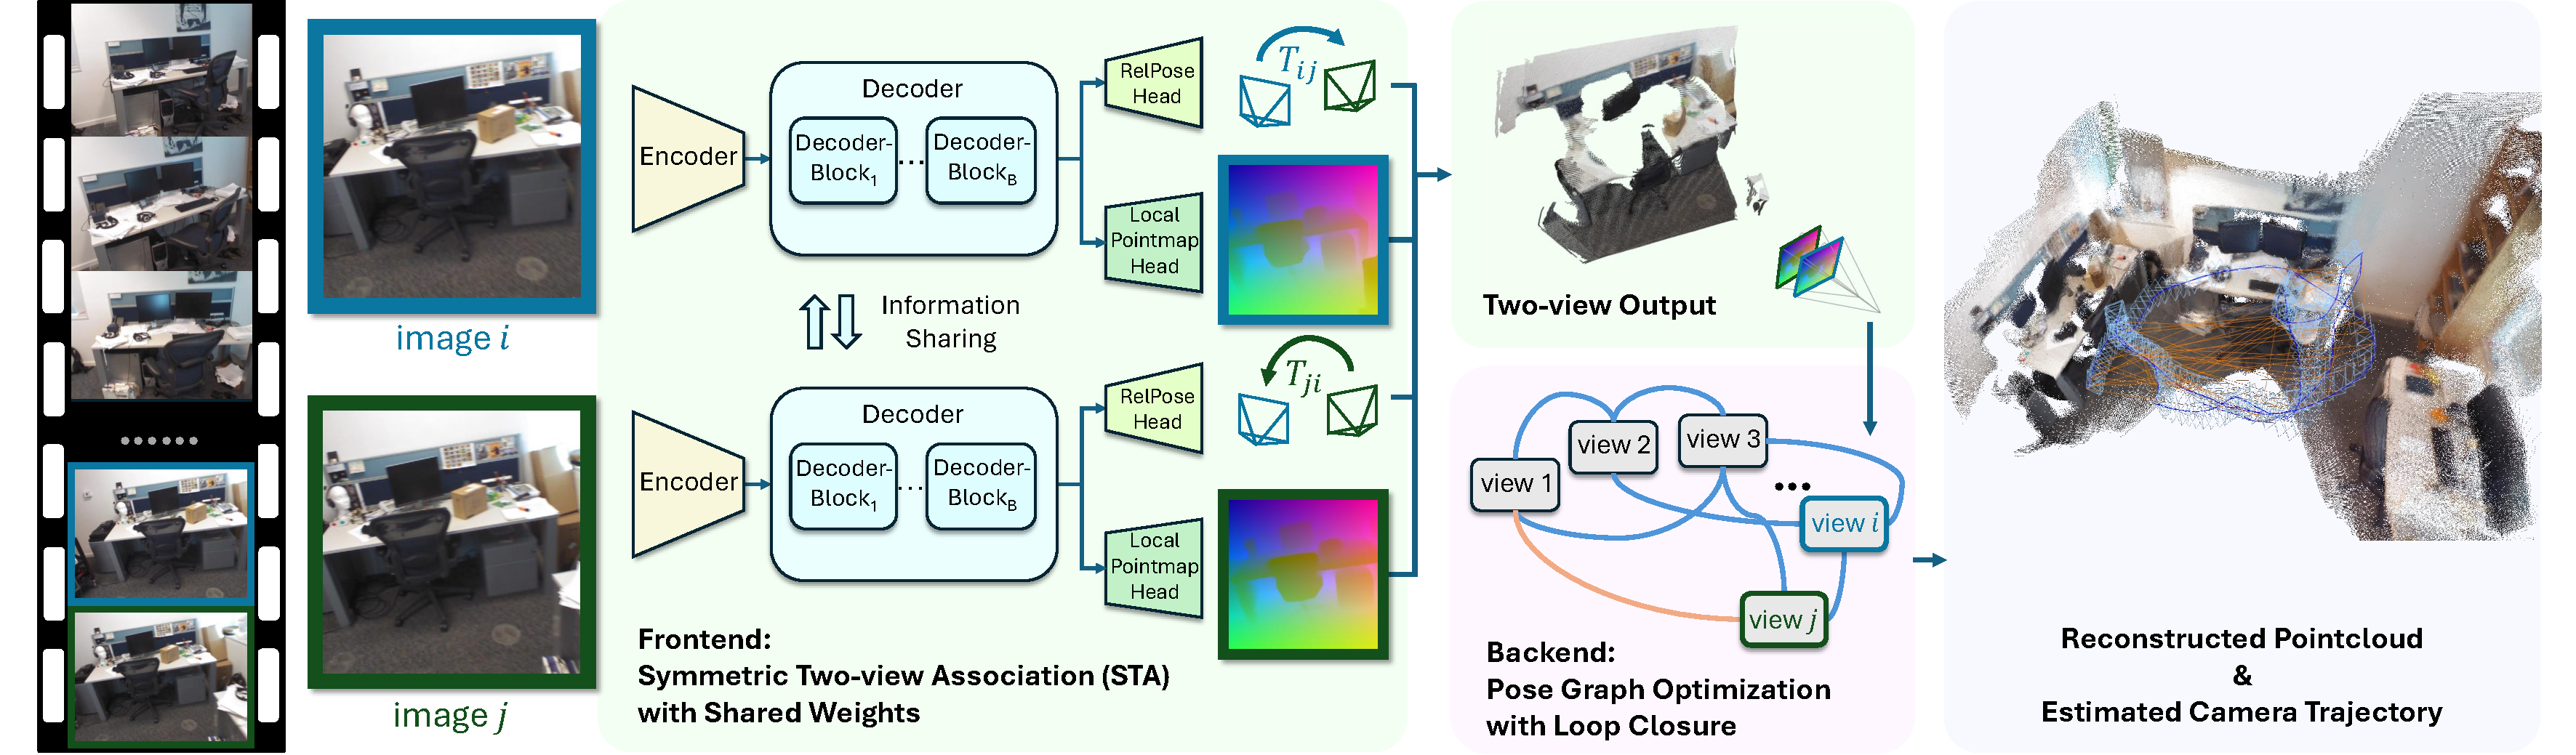
\includegraphics[width=1.0\linewidth]{figs/architecture.pdf}
\caption{\textbf{\ours Overview.} Given sequential video frames without intrinsics as the input, our frontend model takes in view pairs and predicts local pointmaps and relative poses within each pair.
We then use the pair-wise predictions to construct a $\mathrm{Sim(3)}$ pose graph with loop closure and optimize it via Levenberg–Marquardt algorithm. The frontend model employs a fully symmetric design, making the model lightweight and supporting more flexible pose graph optimization. The blue edges in the pose graph and final results represent connections between neighboring nodes (views), while the orange edges correspond to loop closures.}
\label{fig:architecture}
\vspace{-0.5em}
\end{figure*}
